\chapter{Дизајн и архитектура на системот} 

Во претходните два дела беа опишани две различни области кои се основа во
дизајнот и архитектурата на мобилни апликации со знаење за контекстот. Во делот
за пресметување со знаење за контекстот дефиниран е контекстот, опишани се
категориите на различни видови апликации со знаење за контекстот. Притоа опишани
се и неколку софтверски шаблони и рамки по кои треба да се водиме во развојот и
архитектурата на мобилна апликација која сакаме да користи контекстуални
информации. Мобилните социјални мрежи и сервиси се област која во последните
години претрпува огромен развој и трансформации и има огромна улога во
архитектурата и развојот на денешните мобилни апликации. Преку интеграција на
мобилната апликација со овие мрежи и сервиси се обезбедува еден многу значаен
елемент од контекстот на корисниците на мобилната апликација, како што се
неговите пријатели, лични контакти и други социјални врски. Преку овие
информации може да се дознае повеќе и за личните интереси на самиот корисник со
што самата апликација се доближува едно ниво поблиску до корисниците
овозможувајќи високо ниво на персонализација во сервисите кои ги нуди.

\section{Гео Настани} 

Гео Настани е прототип систем преку кој се обидуваме да ги презентираме
опишаните концепти на дизајн и архитектура на апликација со знаење за
контекстот. Системот Гео Настани е замислен како интеграција на веб-сервер,
мобилни клиенти и мобилни социјални мрежи со што се постигнува еден вид мобилен
веб-сервис за организација и промовирање на приватни и јавни настани. Под настан
подразбираме некое случување од каков било вид кое се случува во одредено време,
на одредена локација и е наменето за собирање на група луѓе за одредена цел со
што се постигнува некаков вид на социјализација. Настанот се организира на тој
начин што одреден корисник или повеќе корисници објавуваат јавно или на нивни
пријатели за местото, времето и целта за нивно заедничко собирање и извршување
на групна социјална активност. Денес постојат неколку веб-сервиси кои
овозможуваат организирање и управување на настани како што се Upcoming [59] на
кој себеси се опишуваат како календар на настани, додека Eventful [60] е друг
веб сервис кој им помага на корисниците да пребаруваат, следат и споделуваат
информации за настани. Исто така еден од најпопуларните начини за креирање и
споделување информации за настани е тој што го нуди веб сајтот на социјалната
мрежа Facebook [61] и претежно е наменет за неформални настани организирани и
наменети за сопствениот круг на пријатели. Речиси сите вакви сервиси
овозможуваат креирање, пребарување, споделување информации за приватни или јавни
настани, а некои од нив имаат и мобилни компоненти за кој овозможуваат одредени
функционалности. Во некои од нив се обработува и локацијата на корисникот со што
може да се сметаат и за еден вид на локациски базирани сервиси. Ниту еден од
овие системи не го разработува или вклучува знаењето за контекстот на
корисниците. Во ваков вид на системи, ова знаење може многу да се искористи и да
помогне во подобрување на самите сервиси и генерално подобрување на корисничкото
искуство. Она што системот Гео Настани го поседува во својата архитектура е
мобилната компонента која претставува мобилна апликација што го собира
контекстот на корисникот, соодветно го обработува и извлеченото знаење го
користи да понуди подобар и персонализиран сервис. Притоа оваа мобилна
апликација се интегрира преку еден вид сервисно ориентирана архитектура со
серверската компонента, а се интегрира и со мобилните социјални мрежи со што се
постигнува еден вид модуларна архитектура во кој секоја компонента е независна и
може да биде заменета со друга.

Системот е составен од клиентска мобилна компонента, веб-сервер компонента и
некоја мобилна социјална мрежа. Мобилната компонента е мобилна апликација која
го следи моделот на модуларен дизајн на апликација со знаење за контекстот
сличен на дизајнот со виџети. Серверската компонента од системот ги опслужува
барањата на мобилните клиенти и претставува централно место за интеграција на
мобилната апликација, мобилната социјална мрежа и основен репозиториум на сите
корисници на системот.

\begin{figure}[htb]
\centering
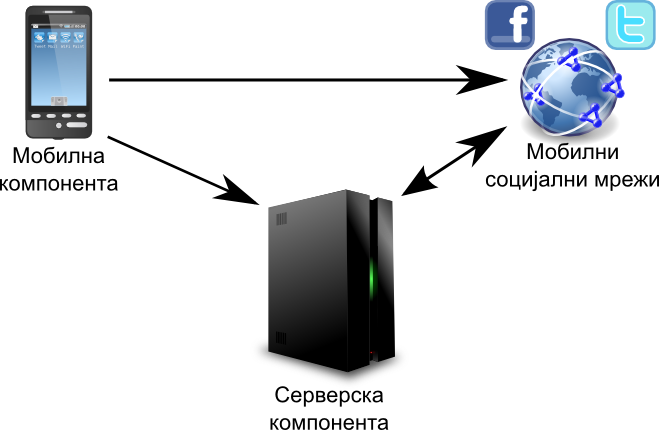
\includegraphics[scale=0.4]{images/architecture}
\caption{Глобална архитектура на Гео Настани}
\label{fig:architecture}
\end{figure}

 
Во центарот на оваа архитектура прикажана на слика 4 е серверската компонента
која ги обединува мобилната компонента и мобилните социјални мрежи. Оваа
компонента е основен дел во сервисно ориентираната архитектура (SOA) и
претставува множество на повеќе REST веб-сервиси кои ги обезбедуваат сите
функционалности кои се потребни во систем за организација на настани. Преку
множеството на веб-сервиси се овозможува креирање на корисници, настани,
пребарување по клучни зборови, локација и се останато што е потребно за
организација на настани од каков било вид. Она што е специфично во оваа
архитектура е што серверската компонента може да се замени со кој било
веб-сервис сличен на погоре споменатите кој обезбедува интерфејс за програмирање
(API) и ги нуди повеќето од можностите потребни за управување со информациите за
настаните.

\begin{figure}[htb]
\centering
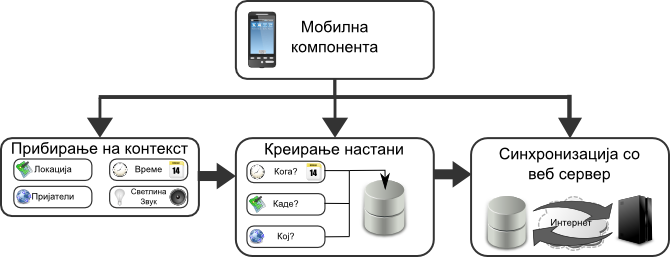
\includegraphics[scale=0.4]{images/mobile_component}
\caption{Архитектура на мобилната компонента на Гео Настани}
\label{fig:mobile_component}
\end{figure}
 
\section{Мобилна компонента}

Мобилната компонента на системот за организација на настани преставува клиентска
мобилна апликација која ги обединува активностите како што се прибирањето на
контекстот, креирањето на настани и синхронизацијата со веб серверот. На
\ref{fig:mobile_component} е прикажана архитектурата на мобилната компонента.
Таа е поделена на три посебни модули: модул за прибирање на контекстот, модул за
креирање настани и модул за синхронизација со веб серверот.

\begin{figure}[htb]
\centering
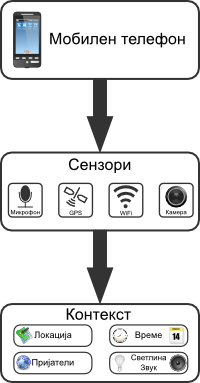
\includegraphics[scale=0.4]{images/context_aquisition}
\caption{Собирање на контекстот во мобилната апликација}
\label{fig:context_aquisition}
\end{figure}

 
Собирањето на контекст е една од најважните компоненти во архитектурата на
мобилна апликација со знаење за контекстот. Во оваа компонента со помош на
користење на соодветни сензори и дополнителни уреди
(\ref{fig:context_aquisition}) се восприемаат информации за контекстот,
соодветно се моделираат и се пренесуваат до релевантните делови од мобилната
апликација.

Следејќи го процесот на развој на апликации со знаење за контекстот прибирањето
на контекстот се одвива со следните неколку чекори: 
\begin{itemize}
  \item Спецификација - во оваа фаза
според доменот на апликација ги извојуваме локацијата, времето, пријателите како
контекст кој треба да се преземе и искористи во апликацијата.
  \item Преземање - за оваа фаза се развиени неколку модули кои ги користат
  соодветните интерфејси за пристап до соодветните сензори и ги преземаат
  потребните информации за конкретниот елемент од контекстот. На пример, за
  локацијата како дел од контекстот тоа може да се моментната локација преку
  латитуда и лонгитуда добиени од интегрираниот GPS уред.
  \item   Испорака и прием - во оваа фаза се моделираат информациите од контекстот и се
  испорачуваат до оние делови во апликацијата за кои се релевантни овие
  информации. За таа цел во модулите од претходната фаза се
моделира контекстот и се обезбедува интерфејс за пристап.
\item Акција - во оваа фаза апликацијата извршува дел од своите предвидени акции но со
дополнително знаење за контекстот преку обработка на информациите примени во
претходната фаза. Со тоа акциите кои се извршуваат се разликуваат во начинот на
извршување предизвикано од самиот контекст.   
\end{itemize}

Креирањето на настани е фазата во која корисникот ги надополнува информациите за
контекстот во кој се наоѓа со цел да се дојде до доволно информации за креирање
на ентитет настан. Ова дополнување на информации означува едноставно додавање на
информации како име на настанот, поместување на времето на настанот или пак може
да биде и модифицирање на некои информации за контекстот како локацијата преку
дополнително опишување. Бидејќи се работи за мобилна апликација наменета за
мобилни уреди, а самите мобилни уреди ги сметаме за доста лични уреди, голема е
веројатноста за одредување на идентитетот на корисникот, односно идентификување
на корисникот со сопственикот на тој мобилен уред. Користејќи го овој значаен
дел од контекстот во фазата на креирање на настани се користи и социјалниот дел
од контекстот составен од листата на контакти која ја поседува самиот корисник.
Откако ќе му се понуди оваа листа со контакти, тој може да изврши дополнително
потпомогнато експлицитно збогатување на контекстот со листа на контакти кои се
поканети на настанот кој го креира, ако се работи за приватен настан.

Во фазата на синхронизација со серверот се одвива целокупната комуникација на
мобилната компонента со серверската компонента во системот. Оваа фаза може да се
извршува на неколку начини и е значајна од неколку аспекти. Нејзиното извршување
може да биде автоматски поттикнато од одредени настани во апликацијата без
знаење на корисникот, а може да се иницира и со конкретна акција за
синхронизација од самиот корисник. Автоматското иницирање се случува кај акции
како креирање на нов настан со цел синхронизација и запазување на интегритетот
на податоците, а се случува и при секое ново стартување на апликацијата со цел
да се започне користење на истата со целосно синхронизирани и ажурирани
податоци. Исто така автоматско иницирање може да се случи и како резултат на
промена на контекстот. Конкретно се работи за дел од контекстот поврзан со
состојбата на поврзаност на мобилниот уред за некоја мобилна мрежа, односно дали
мобилниот телефон има отворена врска со некоја мобилна мрежа и има пристап на
интернет или не е поврзан на мобилна мрежа и не може воопшто да извршува акции
поврзани со синхронизација со серверот. Ако е во состојба на поврзаност акцијата
за синхронизација може автоматски да се стартува.

\section{Одредување на локацијата на корисникот} 

Можноста да се одреди локацијата на корисникот овозможува многу мобилни
апликации да ги прилагодат своите функционалности и сервиси на соодветната
локација и контекст. Знаењето на локацијата на корисникот овозможува апликациите
да им дадат многу поголема точност, а со тоа и вредност на своите сервиси. Денес
луѓето користат локациски базирани апликации во речиси сите сегменти од животот,
како што се забава, навигација, следење на предмети, следење на здравствената
состојба како одговори на ургентни повици и др. Бројот на апликации со знаење на
локацијата на корисникот е во огромен пораст, а се повеќе овие апликации се
развиваат за денешните паметни телефони искористувајќи ги нивните можности за
позиционирање пред сè преку вградените GPS уреди.

Локацијата е еден од најважните елементи на контекстот на корисникот [12].
Покрај тоа што информацијата за локацијата е корисна сама за себе таа може да се
искористи и за одредување на дополнителни информации за контекстот на корисникот
како неговата активност, начинот на транспорт или социјалните врски. На пример,
ако сме повеќе време во сала за вежбање тоа е јасна индикација дека извршуваме
некоја активност поврзана со вежбање, додека ако се движиме со брзина од 90 км/ч
е показател дека се возиме со некое превозно средство.

Информациите за локацијата може да се претстават во апсолутна, релативна или
симболичка форма. Апсолутна локација претставува точна позиција како адреса или
географски координати. Пример, ФЕИТ се наоѓа на ул. „Руѓер Бошковиќ“ б.б.
Релативна локација опишува некоја локација во однос на некоја друга апсолутна
локација. Пример, ФЕИТ се наоѓа околу 3 км западно од Владата на РМ. Симболичка
локација е некое описно име за некоја позната локација како на пример „дома“,
„на работа“ или „во кујна“ и сл. Во повеќето мобилни апликации може да се
користат сите од овие форми на локација, меѓутоа со најголема вредност за
повеќето е апсолутната локација и таа е една од нај-користените форми.

И покрај важноста на информациите за локацијата, сè уште не постои некоја
унифицирана технологија што е прецизна, доволно евтина, лесна за имплементација
и широко распространета. Наместо тоа, постојат колекција од технологии за
лоцирање, при што секоја од нив е за одредена намена, со различни прецизности
која се движи во границите од 1 милиметар со користење на магнетни полиња до
десетици километри со користење на ФМ радио сигнали. Со оглед на тоа што
технологиите за лоцирање се некаков компромис меѓу прецизност и цена, треба да
се избере систем за лоцирање кој ги задоволува потребите на соодветната
апликација. Кај апликациите за мобилни телефони тоа значи дека се избира некоја
од овозможените технологии кои ги нуди самиот телефон или пак се прави
комбинација од сите методи кои ги нуди со помош на некаков софтвер.

\subsection{Карактеристики на технологиите за лоцирање} 

Технологија за лоцирање е комбинација на методи и техники за откривање на
физичката локација на објект или личност во реалниот свет. Локацијата е позиција
во физичкиот простор и како што видовме може да се претстави во апсолутна,
релативна или симболичка форма.

\subsection{Репрезентација на локација} 

Најчестата форма на претставување на прецизна
апсолутна локација е со користење на степените на латитудата и лонгитудата на
точката на површината на Земјата, како што е дефинирано со географскиот
координатен систем. Ако ја земеме Земјата за перфектен елипсоид, со латитудата
се мери аголот меѓу точката и екваторијалната рамнина од центарот на Земјата. Во
реалноста, латитудата, или геодетската латитуда, го мери аголот меѓу екваторот и
линијата која е нормална на референтниот елипсоид, кој ја апроксимира формата на
Земјата. Со лонгитудата го мери аголот меѓу Екваторот и дадената точка. Линијата
која поминува во близина на Кралската обсерваторија, Гринич, Англија, е
прифатена како нулта лонгитуда и е наречена примарен меридијан. Линиите со
константна латитуда се наречени паралели, а линиите со константна лонгитуда се
наречени меридијани. Меридијаните, за разлика од паралелите, не се паралелни и
сите се сечат на Северниот и Јужниот пол. Оваа форма на репрезентација на
локацијата често се користи во локациските системи за отворен простор како што е
GPS. 

Локацијата на Земјата може да се означи и со користење на латитуда и лонгитуда.
На пример, Скопје, Р. Македонија, има латитуда 42\textdegree01$'$ N и лонгитуда
21\textdegree26$'$E. Така, вектор од центарот на Земјата до точката
42\textdegree01$'$ северно од екваторот и 21\textdegree 26$'$ источно од Гринич,
Англија, ќе помине низ Скопје. Со додавање на вертикалното растојание од
центарот на Земјата, или најчесто од средната вредност на нивото на морето на
дадена точка, можно е да се специфицира било која локација под или над
површината на Земјата. Иако географските координати се корисен начин за
определување прецизна апсолутна локација, тие не се соодветни за користење во
апликации кои вклучуваат читање на локациски информации од страна на луѓето.
Ретко може да се случи некој да разбере човек кој би рекол: „Се наоѓам на
30.5432 Север, 65.2344 Запад, или пак дали сакаш да пиеме кафе на 30.552 Север,
64.934 Запад за половина час?“. Како алтернатива, најчесто се користи адреса за
означување локација (на пример, Ул. Маршал Тито 37), симболичко име за местото
познато на двајцата учесници во разговорот (пр. трговскиот центар) или релативни
координати (на пример, 50 метри јужно од мостот). Сервиси за гео-кодирање може
да претвораат адреси и поштенски кодови во географски координати, додека
преведувањето географски координати во адреса или поштенски код може да се
направи со користење на спротивен геокодер. Многу поголем е предизвикот на
одредување локација во затворени простории. Системот може да ја претставува
локацијата во зградата со користење на X и Y растојанијата од одредена фиксна
точка или агол во зградата, додека во зграда со повеќе катови референтна точка
може да се постави на секој кат. Иако ваквиот начин на репрезентација може да е
корисен за системот, сепак вака репрезентираните локации вообичаено се
поврзуваат со концепти на повисоко ниво на симболичка репрезентација, како
„дневна соба“, „спална“, „канцеларија“ или „до автоматот за кафе“.

\begin{figure}[htb]
\centering
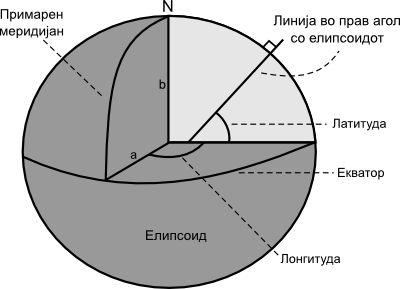
\includegraphics[scale=0.4]{images/gps_coordinates}
\caption{Пример латитуда и лонгитуда на точка на Земјата}
\label{fig:gps_coordinates}
\end{figure}

 
\subsection{Инфраструктура и клиентски базирани системи за лоцирање} 

Генерално постојат три системи за лоцирање: клиентски базирани, мрежно базирани
и мрежно потпомогнати. Во клиентски базиран систем за лоцирање, уредот ја
пресметува сопствената локација без да се потпира на мрежната инфраструктура.
Пример за клиентски базиран систем за лоцирање е GPS, во кој уред опремен со GPS
чип ја пресметува сопствената локација со користење на сигнали кои се примаат од
барем четири GPS сателити.

Во
мрежно базиран систем за лоцирање, мрежната инфраструктура ја пресметува
позицијата на уредот. Пример за мрежно базиран систем за лоцирање е системот
Активна значка [12] во кој значката која ја носат корисниците емитира
инфрацрвени (IR) сигнали кои се примаат од инфрацрвени примачи поставени на
плафонот. Потоа, примачите ги пренесуваат податоците за сигналите до мрежен
процесор кој ја пресметува локацијата на значката. 

Кај мрежно потпомогнатите
системи за лоцирање, и уредот и инфраструктурата учествуваат во пресметувањето
на локацијата на уредот. Пример за мрежно потпомогнат систем за лоцирање е
потпомогнат GPS (A-GPS), во кој уредот ја пресметува сопствената локација врз
база на сопствените GPS мерења и дополнителни информации за констелацијата на
GPS кој се примаат преку линк од мобилната мрежна инфраструктура. Дополнителните
информации му овозможуваат на уредот да ја пресмета сопствената локација и во
недостиг на четири сателити во видното поле и со тоа го намалува времето
потребно за добивање на првата локација. 

Основните предности на клиентски
базиран систем за лоцирање е тоа што ја задржува приватноста на локацијата на
самиот уред. Со тоа што самиот со помош на податоци од инфраструктурата ја
пресметува својата локација без да пренесува податоци, инфраструктурата нема
начин да ја одреди локацијата на уредот, освен ако самиот уред не ги сподели тие
податоци. Од друга страна, пресметување на локацијата на уредот ја троши
батеријата и додава дополнителни барања за пресметковна моќ и големина на
меморија на самиот уред. 

\subsection{Техники за одредување на локацијата} 

Во овој дел се
опишани шест основни техники за одредување на локацијата на уредот: блискост,
трилатерација, хиперболичка трилатерација, триангулација, земање примероци и
пресметување на слепо. Во некои од овие техники се претпоставува претходно
знаење на референтни точки, чија прецизна локација е позната однапред. Примери
за референтни точки се GPS сателит, Wi-Fi пристапна точка (AP) или базна
станица.

\subsubsection{Блискост}  
 
 Чувствувањето на оддалеченоста е нај едноставна техника за
лоцирање. Се користи близината на уредот до референтна точка за да се пресмета
локацијата на уредот. За локација на уредот вообичаено се зема локацијата на
референтната точка. И уредот и референтната точка може да ја чувствуваат
оддалеченоста. Откривање дека некој уред е во близина не имплицира дека се
открива и идентитетот на тој уред, така што за да се открие идентитетот потребен
е посебен механизам. 

Близината може да се открие преку директен физички контакт
или ако уредот се постави во опсегот на една или повеќе референтни точки. На
пример, чекорење врз сензор за притисок означува нечие присуство, а исто така и
комуникација со Wi-Fi пристапна точка означува близина на некој уред до таа
пристапна точка. Во вториот случај, чувствувањето на близината е врз база на
ограничен опсег на покривање на безжичната технологија. На пример, опсегот на
комуникационен уред со мало поле е неколку сантиметри, опсегот на Bluetooth уред
е десетици метри, опсегот на Wi-Fi уред е стотици метри, додека мобилен телефон
може да прима сигнали од базна станица која е оддалечена со километри. Ако
уредот се наоѓа во границите на повеќе референтни точки, можно е да се пресмета
поточна локација. На пример, можно е да се пресмета локацијата на уредот како
просек од позициите на референтните точки. Ако е достапна силината на сигналот
со кој референтните точки го слушаат уредот, може да се пресмета уште по точна
локација со воведување тежини на просеците на референтните точки. 

\subsubsection{Трилатерација}

Трилатерација е техника за лоцирање која ја пресметува позицијата на уредот
преку мерење на растојанијата меѓу уредот и неколку референтни точки на познати
позиции. Бројот на референтни точки потребен за пресметување на локацијата е за
еден поголем од физичката димензија на просторот. На пример, за пресметување на
локација на уред во дводимензионален простор (2-D) потребни се 3 неколинеарни
референтни точки, додека за пресметување на локација во 3-D потребни се четири
референтни точки. 

\begin{figure}[htb]
\centering
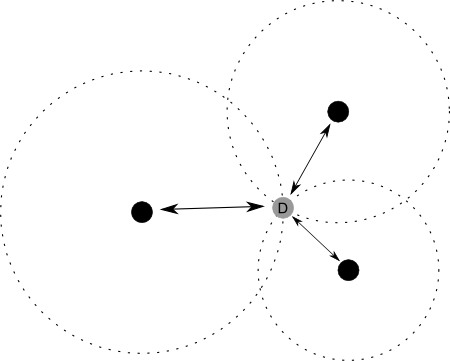
\includegraphics[scale=0.4]{images/trilateration}
\caption{Пример трилатерација во 2-Д. Црните точки претставуваат референтни
точки додека сивата точка е локацијата на уредот.}
\label{fig:trilateration}
\end{figure}

На \ref{fig:trilateration} е прикажана трилатерација во 2-Д. Секоја од црните
точки претставува референтна точка и го дефинира центарот на кругот со радиус
еднаков на пресметаната оддалеченост на уредот. Така, пресметување на
оддалеченоста од една референтна точка дава неограничен број на можни локации на
уредот на периметарот на кружницата. Пресметување на две должини до две
референтни точки дава две можни локации на уредот на пресечните точки на двете
кружници, додека пресметување на три референтни точки единствено ја дефинира
локацијата на уредот. За да се пресмета растојанието меѓу уредот и референтна
точка, често се мери или времето потребно за пристигнување на сигналот или се
мери ослабувањето на силината на сигналот во примачот.
 


\subsubsection{Хиперболичка латерација}

Хиперболичката латерација ја користи разликата на времињата на пристигнување на
сигналите од уредот до три или повеќе референтни точки, наместо да го користи
самото време на патување на сигналот. Техниката на хиперболичка латерација може
да се користи кога уредот прима сигнали кои се симултано испратени од три или
повеќе референтни точки. Во продолжение ќе биде објаснета 2-Д хиперболичка
латерација. Сигналот испратен од уред ќе се прими во различни времиња од
референтни точки на различни позиции на различно растојание од уредот. Разликата
меѓу времињата на пристигнување на сигналот испратен од уредот до две референтни
точки ја ограничува можната локација на уредот на хипербола, при што двете
референтни точки се фокусни точки на хиперболата. На слика 9 е прикажана
хиперболичка латерација во две димензии. Пресекот на двете хиперболи уникатно ја
означува локацијата на уредот.

\begin{figure}[htb]
\centering
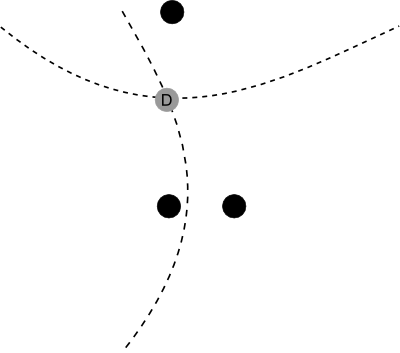
\includegraphics[scale=0.4]{images/trilateration_h}
\caption{Пример хиперболичка латерација во 2-Д. Црните точки претставуваат референтни точки, а сивата точка е локацијата на
уредот.}
\label{fig:trilateration_h}
\end{figure}
 
\begin{figure}[htb]
\centering
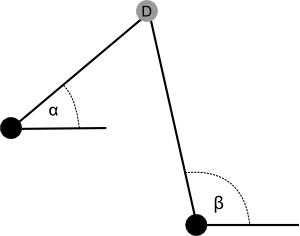
\includegraphics[scale=0.4]{images/triangulation}
\caption{Пример за триангулација во 2-Д. Црните точки претставуваат референтни
точки, а сивата точка е локацијата на уредот.}
\label{fig:triangulation}
\end{figure}

\subsubsection{Триангулација}

 За да се пресмета локацијата на уредот кај триангулацијата се
користи аголот на пристигнување (AOA) на сигналите кој потекнуваат од уредот а
се насочени кон референтните точки. На слика 10 е даден пример на триангулација
во 2-Д. Со мерење на аголот со кој сигналот пристигнува од уредот (преставен со
сива точка) до референтните точки (претставени со црни точки) ја ограничува
позицијата на уредот на линијата која поминува низ референтната точка под аголот
на пристигнување. Мерење на аглите од две референтни точки резултира со две
линии кои уникатно ја дефинираат локацијата на уредот во точката на пресек.
Така, доволно е да се има мерења од само две референтни точки за да се одреди
локацијата на уредот во две димензии, иако често во практиката се користат
повеќе од две референтни точки за да се намалат грешките при мерење. 
За да се
пресмета аголот на пристигнување на сигналот, се користи или насочена антена или
низа од антени. Бидејќи ниту едната ниту другата не се вообичаени за мобилен
уред, најчесто се користат мерењата на референтните точки, кои вообичаено
претставуваат базни станици. 

\subsubsection{Земање примероци} 

Земањето примероци е техника за
локација која користи техники од препознавање на облици за да се пресмета
локацијата на уредот. Иако земањето примероци може да се изведе од многу
различни сензори како што се за звук, светлина и слично, сепак овде ќе го
објасниме со земање примероци на радио сигнали. 

Земањето примероци на радио
сигналите е базирано на две својства на радио сигналите: временска стабилност и
просторна варијабилност. Временска стабилност се однесува на стабилноста на
радио сигналот од одреден радио извор на било која локација во текот на времето.
Јачината на сигналот на одредена локација во тек на времето зависи од јачината
со која сигналот се зрачи од предавателот (која вообичаено е константна) и
апсорпцијата на сигналот од средината (воздух, ѕидови или други препреки).
Просторната варијабилност се однесува на променливоста на радио сигналот од
истиот извор на две различни локации. На пример, силината на сигналот од
непосредната базна станица е различен во канцеларијата и во кафетеријата.
Системите за лоцирање ја земаат предноста на овие две својства преку запишување
на радио профилите на различни физички локации и користење на овие профили за
подоцна да се одреди локацијата. 

Прецизноста на системот за земање примероци е
тесно поврзан со степенот на просторна варијабилност на самиот сигнал. На
пример, силината сигналот од Wi-Fi пристапна точка покажува просторна
варијабилност од 1 до 10 метри, или со други зборови, дадена пристапна точка
може да се слуша посилно или воопшто да не се слуша на неколку метри
оддалеченост. Ова овозможува систем базиран на земање примероци од Wi-Fi
пристапни точки да има околу 1m просторна грешка. 

Многу значајно во земањето
примероци е фазата на тренинг со цел да се изгради радио мапа на целната околина
пред да може да се користи за одредување на локацијата. Во тек на фазата за
тренинг, уредот се движи низ околината, и ја мери силината на сигналот кој се
емитира од група на радио извори (на пример, Wi-Fi пристапни точки). Пример на
радио мерења е даден во Табела 3. Во табелата е прикажана листа со Wi-Fi
пристапни точки и силината на сигналот примен од секоја од пристапните точки.

\begin{table}[!hbp]
\caption{Пример на мерења во кои е вклучено името (SSID), MAC адресата и
силината на сигналот (RSS) од три Wi-Fi пристапни точки}
\begin{tabular}{|p{.3\textwidth} | p{.3\textwidth} | p{.3\textwidth}|}
\hline
SSID (Име) & BSSID (MAC Адреса) & Силина на сигналот (RSS)\\
\hline
ETF WLAN CSD & 00:0e:6a:d3:16:35 & -70\\
\hline
M.F. & 00:23:69:e3:55:e8 & -89\\
\hline
DIPteam & 00:1e:e5:5b:5e:22 & -93\\
\hline
\end{tabular}
\label{tab:samples}
\end{table}

На крајот на фазата за тренинг, системот за земање примероци има радио профил на
повеќе локации во одреден физички простор. Поради тоа што земањето примероци не
ја моделира пропагацијата на радио бранови, прилично густа мрежа на мерења треба
да се собере за да се постигне добра прецизност. Во еден од оригиналните системи
за земање примероци [62], на пример мерењата на силината на сигналот од Wi-Fi се
вршени на 1m оддалеченост. 

Откако ќе заврши фазата со тренинг, уредот може да ја
пресмета сопствената локација со едно мерење и пренесување на резултатите на
системот за земање примероци, кој може да се наоѓа на самиот уреди или на некој
сервер во мрежата. Системот за земање примероци ја пресметува локацијата на
уредот преку пресметување на сличност меѓу моменталните мерења и мерењата
запишани во фазата на тренинг. 

Сличноста меѓу мерењата може да се пресмета на
повеќе начини, меѓутоа често се користи Евклидово растојание во просторот на
сигналите. На пример, ако едно Wi-Fi мерење содржи јачина на сигнали за N
пристапни точки $(S_1, \ldots ,S_n)$ и друго мерење ги содржи мерењата на
јачините на сигналите од истите $N$ извори $(R_1, \ldots ,R_n)$, Евклидовото
растојание меѓу двете мерења се пресметува како:\\
\[
    E = \sqrt{(S_1 - R_1)^2 + \ldots + (S_n - R_n)^2}
\] 

Ако некоја
пристапна точка не е присутна во едно од мерењата, често се заменува јачината на
нејзиниот сигнал или со минималниот сигнал во мерењето или со фиксна
предодредена вредност. 

Постојат повеќе варијации на алгоритмот за земање
примероци. Систем за земање примероци, базиран на алгоритмот за најблизок сосед
$(NN)$ ја пресметува локацијата на уредот како локацијата во мерењата од тренинг
радио профилот со најмало Евклидово растојание од моменталното мерење. Додека со
$k-NN$ алгоритмот се пресметува локацијата на уредот со усреднување на локациите
на $k$ мерења во тренинг профилот со најмалото Евклидово растојание од
моменталното мерење. Идеалното $k$ може да се одреди преку експеримент во
соодветна репрезентативна околина, но мали вредности од 3 до 4 се покажуваат
добро во практика [63].
 
\begin{figure}[htb]
\centering
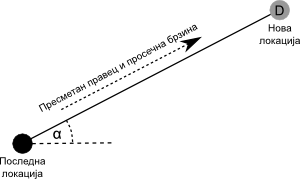
\includegraphics[scale=0.4]{images/dead_reconing}
\caption{Пример на слепо пресметување во 2-Д. Црната точка претставува последно
добиената локација, а сивата претставува пресметаната нова локација.}
\label{fig:dead_reconing}
\end{figure}
 
\subsubsection{Слепо пресметување}

Слепо пресметување е техника за лоцирање која
ја пресметува локацијата на уред на основа неговата претходна локација која е позната,
изминато време од моментот кога е добиена локацијата, правецот и просечната
брзина на движење. Претпоставката  во позадина на слепото пресметување е дека
правецот и просечната брзина на движење од последно добиената локација се или
познати или може да се пронајдат. На \ref{fig:dead_reconing} е илустриран принципот на
слепото пресметување. Црната точка ја претставува последно позната локација на уредот.
Со знаење на овој податок, правецот и просечната брзина, можно е да се пресмета
новата локација на уредот претставена со сивата точка. 

Ограничувањето на ваквото
пресметување е што ја пресметува релативната позиција од последно добиената
локација, така да мора да се користи во комбинација со други технологии за
лоцирање кои имаат можност да ја пресметаат апсолутната локација на уредот.
Слепото пресметување често се користи да се подобрат пресметките од некој друг
систем за лоцирање или да ја пронајдат локацијата кога другиот систем не е
достапен (на пример, кога автомобил влегува во тунел и го губи сигналот од GPS
сателитите). 

Прецизноста на слепото пресметување зависи од квалитетот на
пресметките за брзината и правецот на движење како и прецизноста со која е
одредена почетната локација. Овие вредности може да се добијат преку
екстраполација од две претходни локации или преку мерења од некои сензори на
самиот уред. Некои од сензорите кои често се користат при слепо пресметување се
акцелерометри, кои можат да го измерат забрзувањето на уредот, одометри, кои го
пресметуваат растојанието поминато со автомобил или жироскопи, кои се користат
да го пресметаат правецот на движење. 

\subsection{Можни грешки во одредувањето локација}

Целта на системите за лоцирање е да дадат точна информација за локацијата на
одреден уред, а со тоа и локацијата на корисникот. За жал, во практика,
системите за локација често произведуваат неточни информации поради различни
причини.

\subsubsection{Извори на грешки} 

Системите за лоцирање се дизајнирани да даваат што е можно
поточни информации за локацијата ако мерењата кои ги врши системот се исто така
точни. Сепак, постојат неколку фактори кои воведуваат грешки во системите за
лоцирање. 

\emph{Неточни координати на референтните точки.} Системите за лоцирање на кои
им е потребна прецизна локација на референтните точки продуцираат грешки кога
соодветните локации не се точни. Проблемот може да се избегне или да се реши со
внимателно мапирање на референтните точки. Меѓутоа, за некои референтни точки
кои се мобилни (на пример, GPS сателити) ова може да биде тежок проблем поради
некои неочекувани фактори (на пример, соларни ветрови) кои може да ја променат
локацијата на референтната точка. 

\emph{Јоносферично и тропосферично задоцнување.} Сигналите кои патуваат преку
јоносферата и тропосферата трпат одредени задоцнувања како резултат на интеракциите со атмосферата на Земјата. Иако
постојат математички модели кои се обидуваат да го пресметаат ова задоцнување,
тоа сè уште е причина во поголемиот дел на грешки во GPS базираното
позиционирање. 

\emph{Синхронизација на времињата.} Прецизно мерење на времето побарува
многу прецизна синхронизација меѓу времињата на испраќачот и примачот на
сигналот или меѓу уредите кои испраќаат сигнали истовремено. Постојат алгоритми
за синхронизација кои го намалуваат ефектот на не синхронизирани времиња, но не
ги отстрануваат целосно. Изместувањата на времињата се чести извори на грешки
кај сите системи за лоцирање кои ги користат мерењата на времињата за одредување
на локацијата. 

\emph{Повеќе патишта.} Сигналот кој патува низ просторот може да
пристигне на целната локација преку повеќе различни патишта поради интеракцијата
со пречките на кои може да наиде. Копии на сигналот може да интерферираат пред
да бидат примени од примачот и притоа да имаат дисторзирана амплитуда и фаза.
Ако се нема видлива линија од испраќачот до примачот, проблемите со повеќе
патишта се посериозни и предизвикуваат поголеми грешки во мерењето. 

\emph{Геометрија.} Геометриската конфигурација на референтните точки има голем
ефект на прецизноста. Позиционирање на референтните точки премногу блиску една до друга
или на иста линија вообичаено предизвикува големи грешки во локацијата.

Квалитетот на пресметаната локација која се добива од системот за лоцирање
зависи од повеќе фактори, вклучувајќи ја физичката локација, времето од денот,
моменталните временски околности и атмосферски влијанија како и самата околина.
Така, за целосно да се согледа квалитетот на еден систем за лоцирање, неопходно
е да се соберат голем број на пресметувања на локацијата за разни временски
услови. Процедурата за препознавање на грешките зависи од тоа дали системот
продуцира симболички или апсолутни локации. 

Локациските системи кои симболички
локации, како што се „на работа“ или „дома“, продуцираат резултати кои се или
точни или неточни. Во овој случај, нај често прецизноста се искажува преку
проценти. На пример, систем за лоцирање може да ја погодува собата во некоја
зграда 85\% од времето. Повторување на експериментот повеќе пати овозможува да
се пресмета ниво на доверба на прецизноста на системот. 

Кај системите за лоцирање
кои даваат апсолутни локации, како што се географски координати, вообичаено е да
се прикаже функција на распределба на кумулативна грешка. Во овој случај,
грешката во локацијата е дефинирана како растојанието меѓу вистинската и
пресметаната локација. Исто така често се искажува како 50\% или 95\% грешка во
лоцирањето, кои може да се извадат од функцијата на распределба на кумулативната
грешка. Ако системот работи различно во хоризонтална и вертикална димензија,
тогаш често и грешката се пресметува за секоја димензија. 

\subsubsection{Одредување на локацијата во Гео Настани} 

Како што претходно споменавме денешните
мобилни уреди се опремени со повеќето стандардни системи за лоцирање на корисниците како што е
лоцирање со помош на GPS, лоцирање со триангулација од базни станици, а можно е
и развивање на дополнителни системи за лоцирање. Локацијата несомнено е еден од
најважните елементи од контекстот кој се користи во Гео Настани. Барањата околу
прецизноста на локацијата која го сочинува контекстот на корисникот ја
исполнуваат сите системи за лоцирање достапни во паметните мобилни телефони.
Системот побарува локација во апсолутна форма со незадолжителна информација и за
симболичната форма. Форматот на информацијата за локацијата е латитуда,
лонгитуда и адреса или симболично име на локацијата. Она што е недостаток е
сложеноста на процесот на добивање на локација, затоа што тој зависи од многу
услови во кој корисникот бара да му се одреди локацијата. Сосема се разликува
начинот на одредување локација во отворен и затворен простор. Иако е општо
познато сепак многу малку корисници знаат дека добивање на GPS прецизна локација
во затворен простор е речиси невозможно, или дека добивањето на првичната
локација со помош на триангулација е многу побрзо отколку со GPS системот.
Затоа, во архитектурата на Гео Настани дополнително е развиена компонента за
полесно и интуитивно одредување на локацијата на корисникот. 

Во основа овој
подсистем е комбинација од понудените системи за лоцирање во мобилните телефони,
збогатени со контекстни информации внесени експлицитно од корисникот, како и
постојана можност за избирање на сопствената локација на географска мапа или од
листа од претходно пресметани локации. Исто така додаден е модул за попрецизно
лоцирање во затворени простории кои е базиран на земање примероци од пристапните
точки на постојната Wi-Fi инфраструктура.

\begin{figure}[htb]
\centering
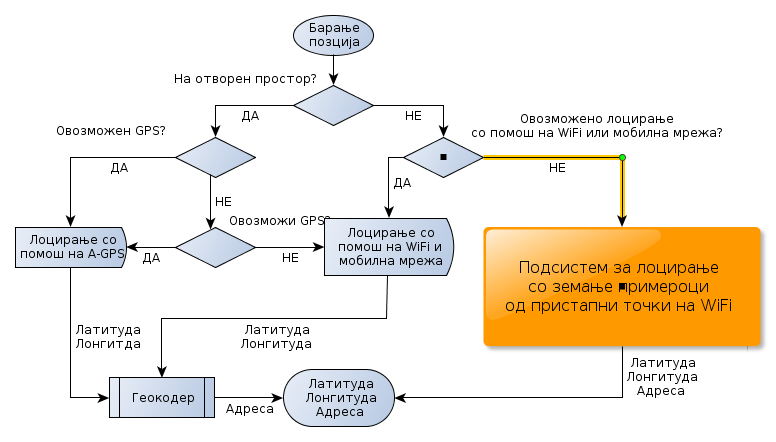
\includegraphics[scale=0.4]{images/locating_flow}
\caption{Дијаграм на активности на процесот на лоцирање на корисникот во
системот Гео Настани.}
\label{fig:locating_flow}
\end{figure}
 
На \ref{fig:locating_flow} е прикажан дијаграмот на активности на модулот
за лоцирање на корисникот во рамките на системот Гео Настани. 

\section{Серверска компонента} 

Серверската компонента е централниот дел во сервисно
ориентираната архитектура (SOA) според која се базира архитектурата на целиот систем. Сервисно
ориентирана архитектура во повеќето случаи се однесува на множество на
веб-сервиси имплементирани преку SOAP или XML-RPC стандардите со цел
комуникација и интеграција на повеќе различни клиенти со еден или повеќе
веб-сервери кои може да се наоѓаат на иста но и на повеќе различни локации. Ако
се погледнат денешните современи веб-системи кои на некој начин имплементираат
сервисно ориентирана архитектура, тоа го прават на малку поинаков начин. Причина
за избегнувањето на SOAP и XML-RPC стандардите е што тие се прилично комплексни
и бараат поголемо познавање на самите протоколи и програмските јазици за нивна
имплементација. Најголемиот дел од популарните веб сервиси своите
функционалности ги прават достапни преку објавување на множество на веб сервиси,
што во програмерскиот свет е по познато како API (интерфејс за програмирање
апликации).

\begin{figure}[htb]
\centering
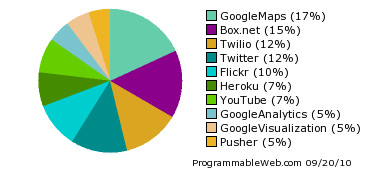
\includegraphics[scale=0.4]{images/web-services}
\caption{Листа на 10 нај користени API достапни на веб}
\label{fig:web-services}
\end{figure}

На \ref{fig:web-services} е дадена листа од нај
користените веб-сервиси на интернет достапни преку соодветно API\footnote{извор
http://www.programmableweb.com/apis}. Кај повеќето
од овие веб-сервиси се следи REST архитектурниот стил со што овој стил на
архитектура во софтверското инженерство е нај застапен во сервисно ориентираните
архитектури на интернет. 

Архитектурата на серверската компонента во Гео Настани
ги следи токму принципите на REST архитектурата. 

Архитектура на REST веб-сервиси REST [64] претставува архитектурен стил за дистрибуиран мрежен систем за
пренесување на ресурси од каков било вид. Во центарот на оваа архитектура се
ресурсите. Сите информации достапни на веб се некаков вид на ресурс. Тоа може да
бидат текстуални информации, слики или каков било друг вид на информации.
Клиентите може да пристапат на овие ресурси преку соодветното URL:
\\[.5cm]
\texttt{http://www.geoevents.mk/event/4321}
\\[.5cm]
по што резултатот што се добива е некаква репрезентација (representation) на
соодветниот ресурс (пр. HTML страница). Оваа репрезентација ја поставува
клиентската апликација во некаква состојба (state). Резултатот од пристапот до
некој друг хиперлинк на HTML страницата ја пренесува клиентската апликација во
друга состојба. Така клиентската апликација ја менува (transfers) состојбата со
секоја различна репрезентација на ресурсот. Според објаснувањето на авторот на
REST „целта е да се добие слика како добро дизајнираните веб апликации се
однесуваат: мрежа од веб страници (виртуелен дискретен автомат), каде
корисниците се движат низ апликацијата преку следење на линкови (транзиција на
состојби), со што како резултат се добива (репрезентација на следната состојба
на апликацијата) следна страница од веб апликацијата“.

\begin{figure}[htb]
\centering
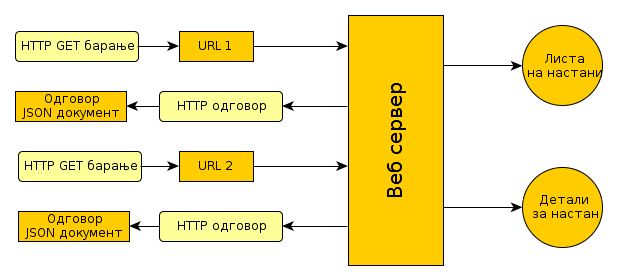
\includegraphics[scale=0.4]{images/rest_architecture}
\caption{REST архитектурен стил на дизајн на веб сервиси}
\label{fig:rest_architecture}
\end{figure}
 
REST претставува стил
на архитектура, а не стандард. Со тоа што не е стандард, не постои никаква
спецификација од некое тело за стандардизирање како W3C или некоја комерцијална
имплементација. Секој кој го следи стилот на оваа архитектура може да ги развие
своите сервиси на REST начин. Всушност многу имплементации на веб-сервиси се
всушност REST без самите да се свесни за тоа. 

Иако REST не е стандард, сепак корисни многу стандарди како:
\begin{itemize}
  \item HTTP
  \item URL
  \item XML/HTML/GIF/JPEG итн (репрезентација на ресурси)
  \item text/xml, text/html, application/json, image/gif, image/jpeg, итн (MIME
видови) 
\end{itemize}
 
Сите ресурси во REST се претставени со некакви логички URL, а секој
ресурс е некаков концептуален ентитет. Репрезентацијата претставува конкретна
манифестација на ресурсот. URL адресата:
\\[.5cm]
\texttt{http://www.geoevents.mk/events/3425}
\\[.5cm]

претставува логичко URL, кое се разликува од физичките URL. Така, може, но не
мора да постои статичка HTML страница за секој настан. Постоење на милиони
настани и милиони статички HTML страници за истите не е атрактивен дизајн.
Самите URL адреси не треба да откриваат никакви детали за техниката на
имплементација која се користи. Треба да имаме можност за менување на
имплементацијата без тоа да се одразува на клиентите или пак да се отстранат не
постоечки URL адреси. 

Некои од позначајните карактеристики на REST веб сервисите се: 
\begin{itemize}
  \item Клиент-сервер - интеракција со повлекување на ресурси (компонентите консументи
консумираат репрезентации на ресурси)
\item Без состојба - секое барање од клиентот до серверот мора да ги содржи сите информации потребни да се разбере
барањето и не може да се земе предвид контекстот на самиот сервер.
\item Кеширање - се зголемува ефикасноста на одговорите, но мора да постои
можноста соодветните ресурси да може да се означуваат дали имаат можност за кеширање или немаат.
\item Стандарден интерфејс – на сите ресурси им се пристапува преку генерички
интерфејс (на пример, HTTP GET, POST, PUT, DELETE)
\item Именувани ресурси - системот
се состои од ресурси кои се именувани со помош на соодветни URL.
\item  Меѓусебно
поврзани репрезентации на ресурси - репрезентациите на ресурсите се поврзани со
користење на URL, така што се овозможува клиентските апликации да ја менуваат
состојбата од една во друга.
\item Слоевити компоненти - медијатори, како што се
прокси сервери, сервери за кеширање, итн, може да се постават меѓу клиентите и
ресурсите за да се зголемат перформансите, сигурноста и сл.
\end{itemize}

Некои од позначајните принципи кои треба да се следат во дизајнот на REST
веб-сервиси се следните:
\begin{enumerate}
  \item Клучот во креирање на успешни веб сервиси во REST мрежа (како што е вебот) е
    да се идентификуваат сите концептуални ентитети кои сакаме да ги објавиме
    преку соодветни сервиси. Примери за такви ентитети во Гео Настани се: листа
    на настани, детали за настанот, место на одвивање на настанот.
    \item Создавање URL за секој ресурс. Ресурсите треба да се именки, а не глаголи. На
пример, лоша практика е да се користи:\\
 \texttt{http://www.geoevents.mk/events/getEvent?id=3425}\\ наместо глаголот
\texttt{getEvent}, треба да се користи именка:
\\\texttt{http://www.geoevents.mk/events/3425}\\
\item Категоризација на
ресурсите во однос на тоа дали клиентите може само да примаат репрезентација на
ресурсите или може да ги менуваат (додаваат нови) ресурси. За оние ресурси кои
може само да се читаат, треба да се овозможи пристап преку HTTP GET, додека за
ресурсите кои може да се менуваат треба да се овозможи HTTP POST, PUT, DELETE.
\item Пристапувањето на ресурси со HTTP GET не треба да предизвикува никакви странични
ефекти. Тоа значи, ресурсот треба само да врати репрезентација на ресурсот.
Повикување на ресурсот не треба да резултира во каква било модификација на ресурсот.
\item  Никој од ресурсите не е остров сам за себе. Со други зборови, треба да
се постават соодветни хиперлинкови во репрезентацијата на ресурсите за да се
овозможи клиентите да преземаат повеќе информации или да дојдат до некои слични
и поврзани информации. 
\item Дизајнирање со цел да се откриваат податоците постепено.
Не треба да се откриваат сите информации во единствен одговор на барањето. Треба
да се овозможат линкови за да се откријат повеќе детали. 
\item Спецификација на форматот на одговорот преку соодветна шема (DTD, W3C
Scheme, RelaxNG или Schematron). За оние сервиси за кои е потребно POST или PUT барање, треба да се
специфицира форматот на барањето. 
\item Опис како треба да се повикуваат сервисите или
преку WSDL документ или преку HTML документ.
\end{enumerate}
    
\subsection{Интеграција со социјални сервиси}

Со големата експанзија на социјалните мрежи, денес речиси и да не постојат луѓе,
пред се од технолошката ера кои не се присутни на некоја социјална мрежа.
Ваквата популарност доведува до огромно количество информации кое може да се
искористи во развојот на апликации. Социјалните мрежи се огромен извор на лични
контекстни информации како што се име, слика, информации за контакт, пол,
љубовен статус, интереси, активности, хоби, музички и филмски вкусови,
припадност на одредени групи и секако информации за поврзаност или пријателство
со други луѓе. Исто така, социјалните мрежи овозможуваат споделување на овие
информации со други корисници, со цел пронаоѓање на луѓе со слични интереси и
нормално воспоставување комуникации со тие луѓе. На социјалните мрежи може да се
гледа како на следниот чекор во природната еволуција на интернет, каде првиот
чекор беше можноста на луѓето да пристапуваат до информации (пример се милијарди
веб-страници со различни информации достапни до секого). За втор чекор во
еволуцијата може да се смета можноста за интеракција на корисниците со веб
сајтовите(пример се можностите за купување производи, создавање лични содржини и
нивно објавување). Следниот значаен и природен чекор е фокусиран на
остварувањето на комуникацијата на луѓето на интернет, а тука несомнено голем
бран предизвикаа многуте социјални мрежи кои успеаја да ги поврзат луѓето и да
им овозможат едноставни можности за директна комуникација и лесно споделување
информации и ресурси.

Интеграцијата на Гео Настани со социјалните мрежи е мотивирана од идејата дека
интегрирањето и прикажувањето на богатството од контекстуални информации од социјалните мрежи во
светот на реална комуникација на корисниците значително може да ја подобри
социјалната интеракција. Да разгледаме едно реално сценарио од системот Гео
Настани. Нека некој корисник присуствува на некој настан од социјален карактер
во кој има можност да остварува комуникација со останатите присутни на тој
настан. Ако во овој случај, на корисникот му се прикажат информации од јавните
социјални профили на другите присутни на настанот, а притоа системот ги
идентификува оние со слични интереси како неговите тој може лесно да ги пронајде
оние корисници со кои би сакал да оствари некој интересен разговор. Ако на
почеток кога го дефиниравме контекстот и рековме дека се тоа информации кои
луѓето ги знаат и лесно ги споделуваат во меѓусебна интеракција, а дека овие
информации потешко се спроведуваат во интеракцијата на луѓето со компјутерите,
сега имаме сосема спротивна ситуација, односно меѓусебната интеракција меѓу
луѓето ја збогатуваме со дигитални контекстни информации од социјалните мрежи на
веб.

\begin{figure}[htb]
\centering
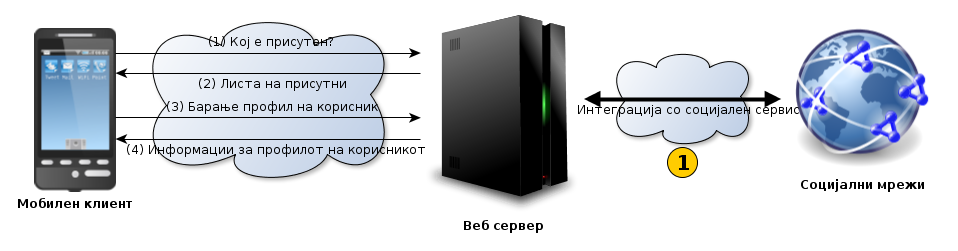
\includegraphics[scale=0.4]{images/social_context_1}
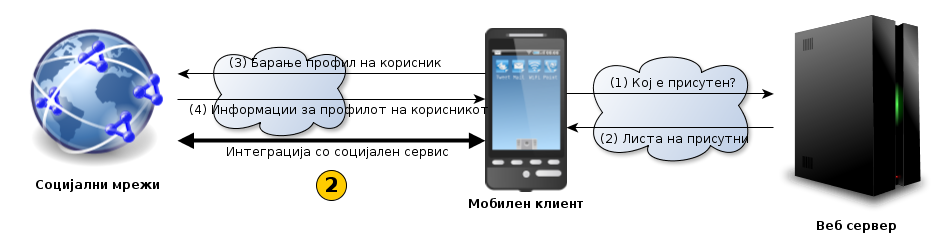
\includegraphics[scale=0.4]{images/social_context_2}
\caption{Две можни точки на интеграција со социјални сервиси во архитектурата
на Гео Настани}
\label{fig:social}
\end{figure}
 

За да се овозможи предложената интеграција во архитектурата на
мобилната апликација и веб серверот потребно е да се пронајдат точките на
интеграција на овие компоненти со социјалните сервиси. На \ref{fig:social} се
прикажани две можни точки на интеграција за конкретното сценарио кога се присуствува на
некој настан. Интеграцијата со социјалните сервиси може да се прави на веб
серверот, но може да се направи и од мобилните клиенти. 

Во првиот случај сите барања за информации поврзани со интеграција со
социјалните сервиси мобилниот клиент ги праќа до веб-серверот на апликацијата,
при што интеграцијата со социјалните сервиси се случува на серверот. Добрата
страна на овој пристап е што на веб-серверот може да се направи кеширање на
податоците од социјалните сервиси и тие не мора да се повикуваат на секое барање
на мобилниот клиент.

Во вториот случај точката на интеграција со социјалните веб-сервиси може да биде
на мобилниот клиент, при што тој ги извршува стандардните барања до веб-серверот
на апликацијата, меѓутоа кога е потребно да се повлечат информации од некој
социјален веб-сервис тоа се прави директно од мобилниот клиент.

Освен предложеното сценарио за интеграција на Гео Настани со социјални
веб-сервиси, можни се и други начини на интеграција со постоечки и популарни
социјални веб сервиси. Интеграцијата се прави за да се овозможат неколку
можности кои додаваат значителен социјален момент во мобилната апликација.
Конкретно преку интеграција се овозможуваат следниве значајни можности:
\begin{itemize}
  \item Споделување на содржини (настани, локации)
  \item Поврзување со корисници на други сервиси
  \item Групирање во групи и заедници со слични и заеднички интереси
  \item Можности за директна комуникација
\end{itemize}
    
  
